\documentclass[10pt,twocolumn,letterpaper]{article}

\usepackage[margin=0.75in,columnsep=0.25in]{geometry}
\usepackage[T1]{fontenc}
\usepackage{lmodern}
\usepackage{microtype}
\usepackage{amsmath,amssymb}
\usepackage{booktabs,tabularx,array}
\usepackage{enumitem}
\usepackage{tikz}
\usetikzlibrary{arrows.meta,positioning,fit,backgrounds}
\usepackage{xcolor}
\usepackage{url}
\usepackage[hidelinks]{hyperref}
\usepackage[font=small,labelfont=bf]{caption}

\newcommand{\sys}{Tanze}
\newcommand{\code}[1]{\texttt{#1}}
\newcommand{\papertitle}{\sys: Evidence-Guided Investigation\texorpdfstring{\\}{ }of CFT Consensus Implementations}
\definecolor{inkblue}{RGB}{35,67,96}
\definecolor{lightblue}{RGB}{237,243,248}
\definecolor{lightgray}{RGB}{246,246,246}
\setlist[itemize]{leftmargin=*,topsep=3pt,itemsep=2pt,parsep=0pt}
\setlength{\emergencystretch}{1em}
\raggedbottom
\urlstyle{same}
\hypersetup{pdftitle={\papertitle},pdfauthor={Yuxin Du}}

\title{\vspace{-1.6em}\Large\bfseries \papertitle}
\author{Yuxin Du\\[0.2em]\normalsize Shanghai Jiao Tong University}
\date{}

\begin{document}
\maketitle

\begin{abstract}
Crash-fault-tolerant (CFT) consensus underpins distributed databases and coordination services, but defects in its implementations can compromise data integrity and service availability. Although LLM agents are increasingly used for code analysis and test generation, they can produce plausible but unsupported reasoning, leading to bug hypotheses based on unverified assumptions or execution histories that violate implementation constraints. Reliable investigation of consensus defects therefore requires grounding suspected violations in source evidence and checking the feasibility of their execution histories. We present \sys{}, an LLM-based system for autonomous investigation of CFT consensus implementations. \sys{} traces the conditions supporting protocol decisions and the progress obligations arising from accepted operations across leadership, membership, and recovery transitions. It combines source-level reasoning with isolated executable experiments to evaluate suspected violations under the implementation's calling and fault assumptions. \sys{} separately records investigation questions, experiment inputs and observations, and interpretations, preserving execution evidence while allowing explanations to be revised. By tracking unresolved premises and explicit dependencies between premises and conclusions, it helps the agent identify claims affected by new evidence and select further source analysis or experiments. \textit{[Evaluation results to be added.]}
\end{abstract}

\section{Introduction}
\label{sec:intro}

Crash-fault-tolerant (CFT) consensus enables distributed databases and coordination services to maintain replicated state despite failures~\cite{raft}. Defects in its implementation can lead to inconsistent data or prevent operations from making progress. Finding such defects requires reasoning across leader election, log replication, persistence, recovery, and membership changes. These components establish conditions that other code paths later rely on. A path that appears correct under its immediate assumptions can behave incorrectly when it uses state or authority from a different protocol context. Investigating the defect requires connecting those paths and determining when their interaction has a consequence for consensus.

LLM agents can explore repositories, formulate bug hypotheses, and construct tests or executable models that are refined using execution feedback~\cite{agora,specula}. Establishing a consensus defect from these artifacts requires tracing the hypothesis's premises to source and checking whether its triggering history respects the implementation's calling and fault assumptions. A plausible explanation can depend on an unexamined producer or reset path; a generated test can supply a state that the implementation cannot reach. Even a completed test may reveal only a local state discrepancy, leaving its effect on agreement or progress unresolved.

The central challenge is to keep a defect hypothesis connected to its supporting premises and observations as the explanation changes, and to use those changes to direct further investigation. Source analysis identifies the protocol responsibility, the history that produces the relevant state, and the observations needed to distinguish competing explanations. Execution can expose a missing premise, contradict the expected effect, or support a narrower conclusion. When new evidence challenges an investigative premise, the agent must identify which conclusions depended on it and reconsider them while preserving the original observations. A source explanation can also resolve a suspicion directly. The revised understanding then determines which unresolved question, source path, or experiment is worth pursuing.

We present \sys{}, an LLM-based system for autonomous investigation of CFT consensus implementations. \sys{} organizes this process around sourced questions that develop through reading, experimentation, and interpretation. To choose what to investigate, the agent traces the conditions supporting protocol decisions and the progress obligations of accepted operations. It follows the paths that create, consume, and restore those conditions across leadership, membership, and recovery transitions. Source reasoning and isolated executable experiments contribute evidence about the histories and consequences of suspected failures.

To support revision, \sys{} separates investigation questions, fixed experimental inputs and observations, and revisable interpretations. An explanation can be corrected using existing evidence; changing an experiment produces a distinct version for fresh execution. Unresolved premises remain attached to their questions. When shared knowledge is corrected, its recorded uses help the agent identify which conclusions require reconsideration. \sys{} returns the updated account and execution results to the same agent session, where the agent chooses whether to trace another source path, refine an experiment, or pursue a new question. This organization connects the evidence behind the current judgment to the choice of subsequent work.

This paper makes three design contributions:
\begin{itemize}
  \item A consensus investigation method that turns decision conditions, progress obligations, and their applicability across protocol transitions into source-grounded questions.
  \item An evidence model that links those questions to exact experiment inputs and observations while keeping interpretations revisable and distinguishing execution outcomes from defect judgments.
  \item A continuation mechanism that exposes unresolved premises and recorded uses of corrected knowledge, helping the agent reconsider affected claims and select further inquiry.
\end{itemize}
\textit{[Evaluation results to be added: evaluated implementations, validated findings, a representative case, and comparative or ablation results supporting the design.]}

\section{Background}
\label{sec:motivation}

Consensus bug discovery combines reasoning about distributed decisions with experiments on executable code. We introduce the correctness properties of consensus implementations and the role of LLM agents in constructing and refining checks of those properties.

\subsection{Consensus implementations}

Consensus enables replicas to agree on decisions despite failures. Replicated state machines use repeated consensus decisions to establish a common sequence of commands, which replicas apply to their local state. Crash-fault-tolerant (CFT) protocols assume that participants follow the protocol until they fail; communication and recovery behavior are governed by the protocol's fault model. In Raft, a leader coordinates log replication, terms distinguish successive election epochs, and voter configurations determine which participants count toward a quorum~\cite{raft}.

Correctness has two complementary aspects. \emph{Safety} excludes inconsistent decisions or effects, such as replicas applying different commands at the same log position. \emph{Liveness} concerns eventual progress under the required availability, scheduling, and communication conditions. For a fixed voter configuration, majority quorums intersect, helping preserve earlier decisions across leader changes. Membership changes and recovery must maintain the conditions on which those decisions depend~\cite{raft}.

An implementation realizes these properties through operations with distinct responsibilities. Receiving a log entry, persisting it, committing it, applying it to a state machine, and completing a client request are different events. Storage, transport, recovery, and asynchronous callbacks connect those events. Investigating an implementation therefore requires understanding both the protocol rule and the code paths that establish its premises. For example, recovery must reconstruct the authority needed for subsequent elections as well as the state needed to resume command execution.

\subsection{LLMs for bug discovery}

LLM coding agents can combine repository exploration with executable analysis. An agent reads source and documentation, proposes a hypothesis about incorrect behavior, constructs a check, and uses the resulting feedback to decide what to inspect or revise next. A bug hypothesis connects a proposed trigger to an expected consequence. An executable test supplies the setup and action sequence, while its \emph{oracle} determines which observed outcomes count as violations. This makes hypothesis construction and test construction closely related tasks~\cite{agora}.

One approach directly generates tests for the implementation. Agora organizes agents around protocol reasoning, scenario construction, and test generation, using consensus knowledge and execution feedback to refine candidate failures~\cite{agora}. Another approach builds an executable abstraction. A model checker explores transitions in a formal model and checks properties such as invariants; a violating trace is a counterexample to the checked property and a candidate implementation failure. Specula uses coding agents to generate specifications, validates models against traces from system code, and attempts to reproduce model-level counterexamples in the implementation~\cite{specula}. These approaches give agents concrete results with which to examine their hypotheses.

Feedback can change more than the generated code. A reproduction failure may reveal a missing precondition, a discrepancy with the model, or an incorrect expectation. A successful check may expose a different mechanism than the one initially suspected. The agent must relate the result to source behavior and revise the corresponding explanation. Iterative investigation thus involves developing the hypothesis, the executable construction, and the meaning of its observations together.

\subsection{Investigation challenges}

For consensus implementations, a useful hypothesis must connect responsibilities distributed across code paths. A vote counts only for an eligible participant and election context; a completion callback must still refer to the operation whose work it finishes. Finding such relationships requires moving between a local behavior and the surrounding producers, consumers, and transitions that give it meaning.

For an execution to support a defect claim, its observations must be connected to an applicable correctness expectation and a permitted history. These elements can evolve as the agent learns more: a newly discovered producer can change the required setup, while an enclosing guard can explain why a suspected failure is prevented. The investigation needs to preserve existing observations, revise the conclusions that depend on changed premises, and use the revised understanding to choose further questions. This motivates \sys{}'s organization around continuing investigations supported by source and execution evidence.

\section{\sys{} Design}
\label{sec:design}

\sys{} takes a captured repository, an execution configuration, and allocations for elapsed time, agent calls, and formal executions. Its objective is to discover and validate sourced defects in CFT consensus, prioritizing safety and progress failures under explicit conditions. The target implementation supplies the source-level responsibilities; the shared method supplies the questions used to investigate them. Target-specific semantic rules are not embedded in the controller.

\subsection{Investigation workflow}
\label{sec:overview}

One native Codex session performs the investigation. The agent can search and read the authorized snapshot, edit draft checks, and obtain permitted local feedback while constructing them. It submits a complete file-backed update that can combine a question, reusable knowledge, an interpretation, and one next execution. The controller checks the submitted structure and references, retains accepted inputs, performs formal execution on a clean isolated source copy, and returns the receipts and current research state to that same session. The captured source and retained evidence remain read-only to the agent. Figure~\ref{fig:architecture} shows the two sources of evidence and the continuing feedback path.

\begin{figure*}[t]
\centering
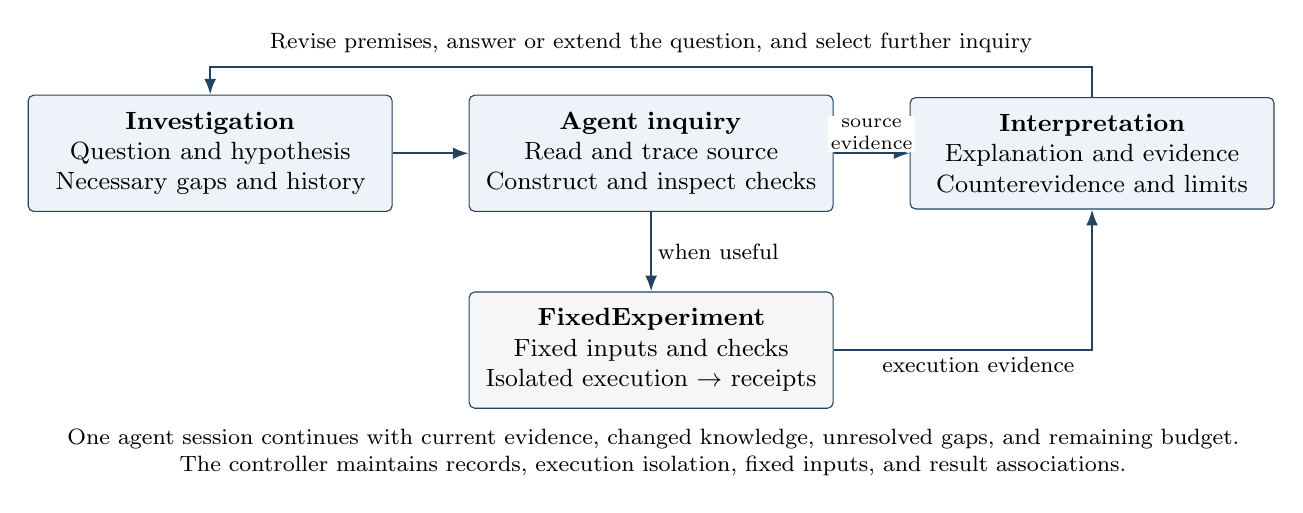
\begin{tikzpicture}[
  n/.style={draw=inkblue,rounded corners=2pt,fill=lightblue,align=center,
    inner sep=6pt,font=\small},
  a/.style={-{Latex[length=2mm]},thick,draw=inkblue},
  lab/.style={font=\footnotesize,fill=white,inner sep=2pt}]
  \node[n,text width=4.2cm] (question) at (0,0) {\textbf{Investigation}\\Question and hypothesis\\Necessary gaps and history};
  \node[n,text width=4.2cm] (reason) at (5.6,0) {\textbf{Agent inquiry}\\Read and trace source\\Construct and inspect checks};
  \node[n,text width=4.2cm] (interpret) at (11.2,0) {\textbf{Interpretation}\\Explanation and evidence\\Counterevidence and limits};
  \node[n,text width=4.2cm,fill=lightgray] (experiment) at (5.6,-2.5) {\textbf{FixedExperiment}\\Fixed inputs and checks\\Isolated execution $\to$ receipts};
  \draw[a] (question) -- (reason);
  \draw[a] (reason) -- node[lab,above,align=center,font=\scriptsize,inner sep=1pt] {source\\evidence} (interpret);
  \draw[a] (reason) -- node[lab,right] {when useful} (experiment);
  \draw[a] (experiment.east) -| node[lab,pos=.28,below] {execution evidence} (interpret.south);
  \draw[a] (interpret.north) -- (11.2,1.1) -- (0,1.1) -- (question.north);
  \node[lab,align=center] at (5.6,1.4) {Revise premises, answer or extend the question, and select further inquiry};
  \node[font=\footnotesize,align=center,text width=15.5cm] at (5.6,-3.8)
    {One agent session continues with current evidence, changed knowledge, unresolved gaps, and remaining budget.\\The controller maintains records, execution isolation, fixed inputs, and result associations.};
\end{tikzpicture}
\caption{Source reasoning and execution contribute to the same investigation. The three semantic objects retain different parts of the inquiry; the agent chooses the next useful action from the resulting explanation.}
\label{fig:architecture}
\end{figure*}

The three objects separate changes that occur at different rates. An \emph{Investigation} owns the sourced question, provisional hypothesis, disposition, necessary gaps, and history. A question may be explained, checked, paused with a resume condition, or split into linked child questions. Its identity persists as the account changes. A \emph{FixedExperiment} records exact harness files and execution inputs, assumptions about scope and history, an optional requirement, and any declared comparisons. An \emph{Interpretation} owns the current account of the whole question, citing source locations and execution receipts and recording counterevidence, answers to gaps, limits, and an explicit defect judgment when one is warranted. A question can receive a source-based interpretation before any experiment exists.

This separation preserves useful work when the investigation changes direction. If a suspected effect has an enclosing protection, the question can be answered from source. If an experiment exposes a missing producer, that premise remains attached to the question while a successor experiment supplies the prefix. If a measurement was misinterpreted, a new interpretation can reuse the unchanged observations. Execution history and the current explanation thus remain distinguishable.

\subsection{Forming questions}
\label{sec:relationships}

\sys{} starts inquiry from a concrete decision or pending duty. The agent identifies what supports it, who produces that support, who consumes it, and which permitted event could change its validity. Two complementary axes guide this reasoning. \emph{Decision formation and progress} asks how eligible support justifies decisions and how accepted work reaches completion, cancellation, or transfer. \emph{Context validity and authority transitions} asks where that support applies and how authority is acquired, transferred, or lost.

\label{sec:example}
For example, consider committed-log replay in HashiCorp Raft~\cite{hashicorp-run}. During startup, replay advances \code{lastApplied}, and a later membership scan starts after \(\max(\mathit{snapshotIndex},\mathit{lastApplied})\). A configuration entry passed by replay can therefore be skipped by the scan while the node retains the snapshot's older voter set. The investigative question is whether recovered application progress also establishes the membership needed for an election. Answering it connects the producer of the progress marker, the scan that consumes it, and the voter set used by election logic.

Five supporting mechanisms locate the responsibilities through which these relationships are realized (Table~\ref{tab:mechanisms}). They overlap: persistence can preserve an election premise, and client completion can expose a safety failure. The agent follows the relevant producers and consumers through admission, dispatch, reset, and completion, preserving materially different failure and asynchronous paths. Broad orientation and local tracing refine each other; a sourced local question can begin before a global map or a settled correctness requirement exists.

\begin{table}[t]
\caption{Supporting mechanisms connect consensus relationships to implementation responsibilities.}
\label{tab:mechanisms}
\small
\setlength{\tabcolsep}{4pt}
\begin{tabularx}{\columnwidth}{@{}>{\raggedright\arraybackslash}p{0.35\columnwidth}>{\raggedright\arraybackslash}X@{}}
\toprule
Mechanism & Responsibility to investigate \\
\midrule
Recovery and resynchronization & Restore the state needed for eligible participation. \\
Configuration and participant eligibility & Establish whose support counts in the current context. \\
Decision application and consumption & Preserve the identity, order, and effects of decisions. \\
History and persistence & Retain or reconstruct the premises used by later decisions. \\
Client contracts and completion & Connect accepted duties to invocation intervals and observable endpoints. \\
\bottomrule
\end{tabularx}
\end{table}

A provisional hypothesis predicts a difference that would matter to the question. Its discriminator identifies information that could still change the judgment: an untraced producer, a reset path, a calling restriction, or an observable endpoint. Uncertainty about the applicable responsibility is itself a valid subject of inquiry. The agent distinguishes normative expectations from implementation behavior, assertions, assumptions, and observations before deciding what a check should establish.

Source reasoning can also resolve the suspicion. In an etcd Raft investigation, the agent asked whether a delayed append rejection could lower the leader's next replication index for a follower while tracking that follower in snapshot state~\cite{etcd-run}. The rejection path can change the index, but the send path treats snapshot state as paused and returns before using it. Both snapshot-success and snapshot-failure paths subsequently enter probe state and reconstruct the next index from matched progress and any retained pending snapshot. Tracing these consumers and transitions explained why the suspected regressed value did not drive the proposed send along those paths. The account was source-based and required no executable witness.

When a source explanation becomes useful elsewhere or needs durable correction, the agent records it as reusable knowledge. A \emph{Behavior} describes actual conditional execution, including ordering, guards, state changes, and completion. A \emph{Fact} states what those behaviors establish for a specified object and context under explicit conditions. Uses refer to a particular revision and can identify the assertion being relied on. These records support reuse as the investigation develops.

\subsection{Building executable evidence}
\label{sec:evidence}

\textbf{Establish the applicable history.}
An execution becomes informative when its construction supplies the premises of the question. The agent traces decisive inputs to permitted producers and identifies what the environment or caller must provide. It can start with a focused handler call or supplied state to explore a mechanism. When a consequence depends on how that state arose, the next step is to construct the relevant prefix, identify an enclosing protection, or retain the missing history as a necessary gap. Real constructors, in-process nodes, memory transports, and target test facilities can supply such a history when they preserve the relevant protocol and calling conditions.

In the recovery investigation, an initial cluster trial recorded a persisted commit index of zero and did not reproduce stale membership. The agent traced the value to \code{tryStageCommitIndex}, which stages it only while \code{RestoreCommittedLogs} is enabled. Enabling the feature only at restart had omitted a necessary premise. The next experiment enabled it during the initial execution and produced the persisted state through the implementation before exercising recovery.

Figure~\ref{fig:case} shows the resulting history, constructed through cluster initialization, snapshots, and \code{AddVoter} calls. A snapshots voters $\{A,B,C\}$ at index 6, then persists commit index 8 after the cluster has expanded to five voters. On restart, replay advances A's applied index to 8 but leaves its voter set unchanged. Partitioning $\{A,C\}$ from $\{B,D,E\}$ allows A to elect itself with two votes and B with three. C still recognizes A as an eligible candidate, while A evaluates the votes against its stale threshold. Both leaders' \code{Apply} futures complete successfully for different commands at index 11. The experiment uses in-memory stores and transports, shortened timeouts, and a graceful restart from retained stores.

\begin{figure}[t]
\centering
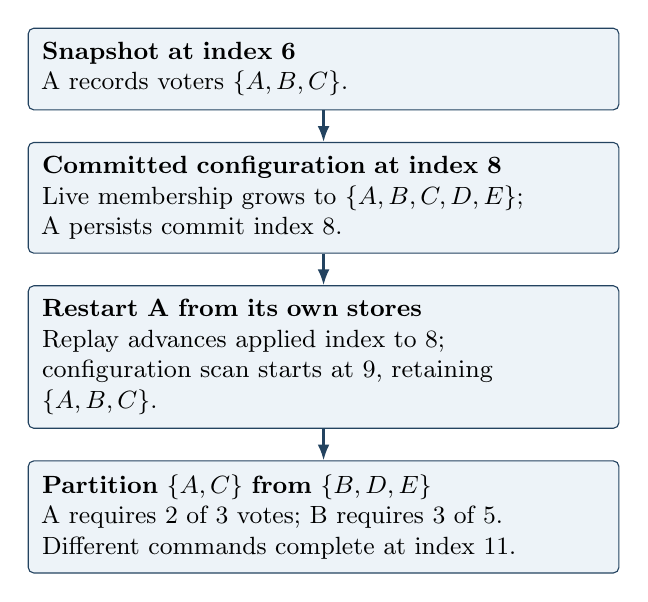
\begin{tikzpicture}[
  box/.style={draw=inkblue,rounded corners=2pt,fill=lightblue,
    align=left,text width=7.15cm,inner sep=5pt,font=\small},
  edge/.style={-{Latex[length=2mm]},thick,draw=inkblue}]
  \node[box] (snapshot) {\textbf{Snapshot at index 6}\\A records voters $\{A,B,C\}$.};
  \node[box,below=4mm of snapshot] (grow) {\textbf{Committed configuration at index 8}\\Live membership grows to $\{A,B,C,D,E\}$;\\A persists commit index 8.};
  \node[box,below=4mm of grow] (restart) {\textbf{Restart A from its own stores}\\Replay advances applied index to 8;\\configuration scan starts at 9, retaining $\{A,B,C\}$.};
  \node[box,below=4mm of restart] (split) {\textbf{Partition $\{A,C\}$ from $\{B,D,E\}$}\\A requires 2 of 3 votes; B requires 3 of 5.\\Different commands complete at index 11.};
  \draw[edge] (snapshot) -- (grow);
  \draw[edge] (grow) -- (restart);
  \draw[edge] (restart) -- (split);
\end{tikzpicture}
\caption{A recorded producer history connects recovery to conflicting commits. A later sample reads stored entries directly: both commands occupy index 11, term 3, and have been applied to their respective state machines.}
\label{fig:case}
\end{figure}

\textbf{Observe the endpoint that bears on the question.}
The agent inspects how the harness obtains each decisive value, following it from the runtime object through a callback, return, or sample. The comparison must use independently identified operations or objects, actual operands, and the relevant ordering. In the recovery example, the first write-term measurement sampled a node's current term after \code{Apply}. An extended execution instead read the stored entry terms and state-machine contents after healing the partition: A and C retained and had applied one command at index 11, term 3, while B, D, and E retained and had applied the other. Together with the successful \code{Apply} completions, these observations establish conflicting commits and divergent applied state. Each endpoint answers a distinct part of the question.

Fixed experiments can declare machine-readable comparisons over emitted observations. A comparison specifies the relevant events, admission and prerequisite relationships, identity fields, applicability conditions, and the fields or constants to compare. The controller associates observations through these declared relationships and checks comparison results. The field under comparison cannot also determine its identity or applicability. Missing fields, unobserved prerequisites, ambiguous associations, and admitted operations with missing completions remain unresolved. This prevents the comparison machinery from turning absent evidence into an expected value.

These checks operate on the declared observations. The agent remains responsible for establishing that the instrumentation measures the intended event and that the stated history and prerequisites suffice. It uses source inspection, raw output, and observations that distinguish competing explanations. For example, a test-authored boolean saying that a minority committed is insufficient if no write was issued; the operation's invocation, completion, and stored effect supply the relevant basis. A control or an additional execution is useful when it resolves a concrete uncertainty about that basis.

\textbf{Separate execution, comparison, and defect judgment.}
\sys{} records whether execution completed, whether a declared predicate held, and what defect explanation the evidence supports. These judgments answer different questions. A predicate predicting that restarted membership equals the old snapshot can hold and support a defect claim. A successful test process can contain no applicable observation of the suspected operation. Requirement-free exploratory executions can produce observations that later receive a sourced interpretation.

An interpretation therefore names its sources and receipt observations and explains their bearing on the whole question. It preserves counterevidence and states the scope of any asserted, refuted, or unresolved defect claim. When an argument links a producer history from one experiment to observations from another, the agent explains their joint-history compatibility. A local answer establishes only its own responsibility: demonstrating stale recovered membership leaves its consensus consequence open until the additional history and endpoints support it. Similarly, a bounded progress claim needs a permitted trigger, actual opportunities to progress, and an explanation of the retry, rejection, or reset behavior under the stated conditions.

Failures, cancellations, timeouts, and incomplete observations remain attached to their receipts. Interpretation can preserve an independently completed witness while keeping missing admissions, completions, and failed scenarios unresolved.

\subsection{Revision and continuation}
\label{sec:continuation}

\textbf{Correct the explanation at its point of dependence.}
New evidence can defeat a premise, limit a consequence, or exclude one candidate cause. The agent updates the question's current interpretation accordingly, retaining the previous accounts and their observations. Necessary gaps record unresolved issues in applicability, producer history, measurement, or causal attribution. Answers identify the specific gap, explain their basis, and explicitly mark it resolved or unresolved. A later answer can reopen the gap without removing its earlier answers. A child investigation's result contributes evidence to its parent, whose broader question still requires its own explanation.

When a reusable premise changes, \sys{} exposes its recorded direct and derived uses, including uses of earlier revisions. The agent identifies which uses depend on the changed assertion and why. Those affected uses become explicit reconsideration points under the corresponding investigations, while independent support remains available. The controller validates the recorded references and retains the revision history; selecting the substantively affected uses is part of the agent's reasoning. A newly discovered dependence can also be recorded directly as a necessary gap in an existing question.

\textbf{Preserve observations across revisions.}
A corrected interpretation can cite the same inputs and receipts. Changing an explanation therefore does not require changing a harness or rerunning an unchanged execution. When the requirement, harness, applicability conditions, observation, or comparison changes, the method calls for a successor experiment with its predecessor, actual difference, and a fresh execution. The controller checks a declared predecessor and retains both versions. Rejected submissions return their full draft and diagnostics for repair, keeping the surrounding research context available.

\textbf{Select the next useful action from the revised account.}
After an interpretation, a pause, or an unchanged update, the same session receives current result locations, outstanding gaps, changed knowledge, and remaining allocation. The agent can pursue a consequential missing premise, trace another path that maintains it, or open an independent sourced question. The latest test and the existing question list do not delimit the search. A source explanation can free attention for another relationship; a counterexample can expose a new responsibility to investigate.

The controller maintains the exact session identity across these exchanges. An open run continues until its configured time or call boundary, or an actual interruption. A preconfigured finite directed task can finish when its specified work is complete. Formal execution has a separate allocation, so source analysis and interpretation can continue when no executions remain. Near a boundary, a saved receipt, an unresolved source path, or a correction may offer useful work within the available time. The continuation mechanism preserves the opportunity and context for such inquiry; the agent chooses which action is likely to change the judgment.

The retained output is an inspectable research history: current questions and explanations, exact experiment versions and receipts, reusable knowledge with recorded uses, and unresolved premises for later work. Together, these artifacts connect what the system investigated, what its executions observed, and the recorded reasoning behind its current claims.

\bibliographystyle{unsrt}
\bibliography{references}

\end{document}
